\chapter{Range queries}

\index{range query}
\index{sum query}
\index{minimum query}
\index{maximum query}

In a \key{range query}, a range of an array
is given and we should calculate some value from the
elements in the range. Typical range queries are:
\begin{itemize}
\item \key{sum query}: calculate the sum of elements in range $[a,b]$
\item \key{minimum query}: find the smallest element in range $[a,b]$
\item \key{maximum query}: find the largest element in range $[a,b]$
\end{itemize}
For example, in range $[4,7]$ of the following array,
the sum is $4+6+1+3=14$, the minimum is 1 and the maximum is 6:
\begin{center}
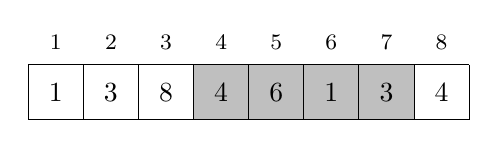
\begin{tikzpicture}[scale=0.7]
\fill[color=lightgray] (3,0) rectangle (7,1);
\draw (0,0) grid (8,1);

\node at (0.5,0.5) {$1$};
\node at (1.5,0.5) {$3$};
\node at (2.5,0.5) {$8$};
\node at (3.5,0.5) {$4$};
\node at (4.5,0.5) {$6$};
\node at (5.5,0.5) {$1$};
\node at (6.5,0.5) {$3$};
\node at (7.5,0.5) {$4$};

\footnotesize
\node at (0.5,1.4) {$1$};
\node at (1.5,1.4) {$2$};
\node at (2.5,1.4) {$3$};
\node at (3.5,1.4) {$4$};
\node at (4.5,1.4) {$5$};
\node at (5.5,1.4) {$6$};
\node at (6.5,1.4) {$7$};
\node at (7.5,1.4) {$8$};
\end{tikzpicture}
\end{center}

An easy way to answer a range query is
to iterate through all the elements in the range.
For example, we can answer a sum query as follows:

\begin{lstlisting}
int sum(int a, int b) {
    int s = 0;
    for (int i = a; i <= b; i++) {
        s += t[i];
    }
    return s;
}
\end{lstlisting}

The above function handles a sum query
in $O(n)$ time, which is slow if the array is large
and there are a lot of queries.
In this chapter we will learn how
range queries can be answered much more efficiently.

\section{Static array queries}

We will first focus on a simple case where
the array is \key{static}, i.e.,
the elements never change between the queries.
In this case, it suffices to process the
contents of the array beforehand and construct
a data structure that can be used for answering
any possible range query efficiently.

\subsubsection{Sum query}

\index{prefix sum array}

Sum queries can be answered efficiently
by constructing a \key{sum array}
that contains the sum of the range $[1,k]$
for each $k=1,2,\ldots,n$.
After this, the sum of any range $[a,b]$ of the
original array
can be calculated in $O(1)$ time using the
precalculated sum array.

For example, for the array
\begin{center}
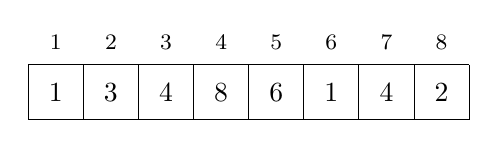
\begin{tikzpicture}[scale=0.7]
%\fill[color=lightgray] (3,0) rectangle (7,1);
\draw (0,0) grid (8,1);

\node at (0.5,0.5) {$1$};
\node at (1.5,0.5) {$3$};
\node at (2.5,0.5) {$4$};
\node at (3.5,0.5) {$8$};
\node at (4.5,0.5) {$6$};
\node at (5.5,0.5) {$1$};
\node at (6.5,0.5) {$4$};
\node at (7.5,0.5) {$2$};

\footnotesize
\node at (0.5,1.4) {$1$};
\node at (1.5,1.4) {$2$};
\node at (2.5,1.4) {$3$};
\node at (3.5,1.4) {$4$};
\node at (4.5,1.4) {$5$};
\node at (5.5,1.4) {$6$};
\node at (6.5,1.4) {$7$};
\node at (7.5,1.4) {$8$};
\end{tikzpicture}
\end{center}
the corresponding sum array is as follows:
\begin{center}
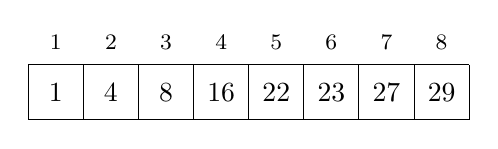
\begin{tikzpicture}[scale=0.7]
%\fill[color=lightgray] (3,0) rectangle (7,1);
\draw (0,0) grid (8,1);

\node at (0.5,0.5) {$1$};
\node at (1.5,0.5) {$4$};
\node at (2.5,0.5) {$8$};
\node at (3.5,0.5) {$16$};
\node at (4.5,0.5) {$22$};
\node at (5.5,0.5) {$23$};
\node at (6.5,0.5) {$27$};
\node at (7.5,0.5) {$29$};


\footnotesize
\node at (0.5,1.4) {$1$};
\node at (1.5,1.4) {$2$};
\node at (2.5,1.4) {$3$};
\node at (3.5,1.4) {$4$};
\node at (4.5,1.4) {$5$};
\node at (5.5,1.4) {$6$};
\node at (6.5,1.4) {$7$};
\node at (7.5,1.4) {$8$};
\end{tikzpicture}
\end{center}
The following code constructs a prefix sum
array \texttt{s} from array \texttt{t} in $O(n)$ time:
\begin{lstlisting}
for (int i = 1; i <= n; i++) {
    s[i] = s[i-1]+t[i];
}
\end{lstlisting}
After this, the following function answers
a sum query in $O(1)$ time:
\begin{lstlisting}
int sum(int a, int b) {
    return s[b]-s[a-1];
}
\end{lstlisting}

The function calculates the sum of range $[a,b]$
by subtracting the sum of range $[1,a-1]$
from the sum of range $[1,b]$.
Thus, only two values from the sum array
are needed, and the query takes $O(1)$ time.
Note that thanks to the one-based indexing,
the function also works when $a=1$ if $\texttt{s}[0]=0$. 

As an example, consider the range $[4,7]$:
\begin{center}
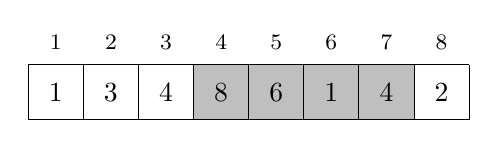
\begin{tikzpicture}[scale=0.7]
\fill[color=lightgray] (3,0) rectangle (7,1);
\draw (0,0) grid (8,1);

\node at (0.5,0.5) {$1$};
\node at (1.5,0.5) {$3$};
\node at (2.5,0.5) {$4$};
\node at (3.5,0.5) {$8$};
\node at (4.5,0.5) {$6$};
\node at (5.5,0.5) {$1$};
\node at (6.5,0.5) {$4$};
\node at (7.5,0.5) {$2$};

\footnotesize
\node at (0.5,1.4) {$1$};
\node at (1.5,1.4) {$2$};
\node at (2.5,1.4) {$3$};
\node at (3.5,1.4) {$4$};
\node at (4.5,1.4) {$5$};
\node at (5.5,1.4) {$6$};
\node at (6.5,1.4) {$7$};
\node at (7.5,1.4) {$8$};
\end{tikzpicture}
\end{center}
The sum of the range $[4,7]$ is $8+6+1+4=19$.
This can be calculated from the sum array
using the sums $[1,3]$ and $[1,7]$:
\begin{center}
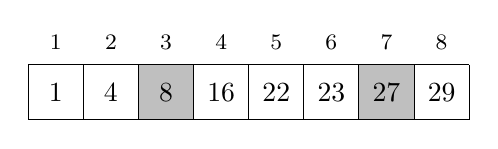
\begin{tikzpicture}[scale=0.7]
\fill[color=lightgray] (2,0) rectangle (3,1);
\fill[color=lightgray] (6,0) rectangle (7,1);
\draw (0,0) grid (8,1);

\node at (0.5,0.5) {$1$};
\node at (1.5,0.5) {$4$};
\node at (2.5,0.5) {$8$};
\node at (3.5,0.5) {$16$};
\node at (4.5,0.5) {$22$};
\node at (5.5,0.5) {$23$};
\node at (6.5,0.5) {$27$};
\node at (7.5,0.5) {$29$};


\footnotesize
\node at (0.5,1.4) {$1$};
\node at (1.5,1.4) {$2$};
\node at (2.5,1.4) {$3$};
\node at (3.5,1.4) {$4$};
\node at (4.5,1.4) {$5$};
\node at (5.5,1.4) {$6$};
\node at (6.5,1.4) {$7$};
\node at (7.5,1.4) {$8$};
\end{tikzpicture}
\end{center}
Thus, the sum of the range $[4,7]$ is $27-8=19$.

We can also generalize the idea of a sum array
for a two-dimensional array.
In this case, it will be possible to calculate the sum of
any rectangular subarray in $O(1)$ time.
The sum array will contain sums
for all subarrays that begin from the upper-left corner.

\begin{samepage}
The following picture illustrates the idea:
\begin{center}
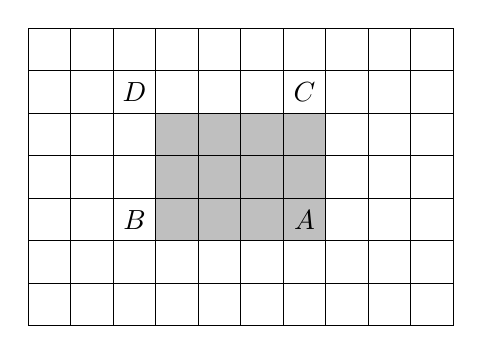
\begin{tikzpicture}[scale=0.54]
\draw[fill=lightgray] (3,2) rectangle (7,5);
\draw (0,0) grid (10,7);
%\draw[line width=2pt] (3,2) rectangle (7,5);
\node[anchor=center] at (6.5, 2.5) {$A$};
\node[anchor=center] at (2.5, 2.5) {$B$};
\node[anchor=center] at (6.5, 5.5) {$C$};
\node[anchor=center] at (2.5, 5.5) {$D$};
\end{tikzpicture}
\end{center}
\end{samepage}

The sum inside the gray subarray can be calculated
using the formula
\[S(A) - S(B) - S(C) + S(D)\]
where $S(X)$ denotes the sum in a rectangular
subarray from the upper-left corner
to the position of letter $X$.

\subsubsection{Minimum query}

It is also possible to answer a minimum query
in $O(1)$ time after preprocessing, though it is
more difficult than answer a sum query.
Note that minimum and maximum queries can always
be implemented using same techniques,
so it suffices to focus on the minimum query.

The idea is to find the minimum element for each range
of size $2^k$ in the array.
For example, in the array

\begin{center}
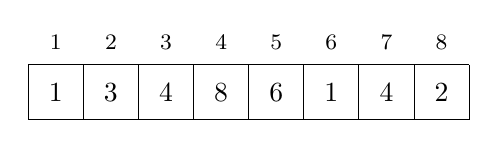
\begin{tikzpicture}[scale=0.7]
\draw (0,0) grid (8,1);

\node at (0.5,0.5) {$1$};
\node at (1.5,0.5) {$3$};
\node at (2.5,0.5) {$4$};
\node at (3.5,0.5) {$8$};
\node at (4.5,0.5) {$6$};
\node at (5.5,0.5) {$1$};
\node at (6.5,0.5) {$4$};
\node at (7.5,0.5) {$2$};

\footnotesize
\node at (0.5,1.4) {$1$};
\node at (1.5,1.4) {$2$};
\node at (2.5,1.4) {$3$};
\node at (3.5,1.4) {$4$};
\node at (4.5,1.4) {$5$};
\node at (5.5,1.4) {$6$};
\node at (6.5,1.4) {$7$};
\node at (7.5,1.4) {$8$};
\end{tikzpicture}
\end{center}
the following minima will be calculated:

\begin{center}
\begin{tabular}{ccc}

\begin{tabular}{ccc}
range & size & min \\
\hline
$[1,1]$ & 1 & 1 \\
$[2,2]$ & 1 & 3 \\
$[3,3]$ & 1 & 4 \\
$[4,4]$ & 1 & 8 \\
$[5,5]$ & 1 & 6 \\
$[6,6]$ & 1 & 1 \\
$[7,7]$ & 1 & 4 \\
$[8,8]$ & 1 & 2 \\
\end{tabular}

&

\begin{tabular}{ccc}
range & size & min \\
\hline
$[1,2]$ & 2 & 1 \\
$[2,3]$ & 2 & 3 \\
$[3,4]$ & 2 & 4 \\
$[4,5]$ & 2 & 6 \\
$[5,6]$ & 2 & 1 \\
$[6,7]$ & 2 & 1 \\
$[7,8]$ & 2 & 2 \\
\\
\end{tabular}

&

\begin{tabular}{ccc}
range & size & min \\
\hline
$[1,4]$ & 4 & 1 \\
$[2,5]$ & 4 & 3 \\
$[3,6]$ & 4 & 1 \\
$[4,7]$ & 4 & 1 \\
$[5,8]$ & 4 & 1 \\
$[1,8]$ & 8 & 1 \\
\\
\\
\end{tabular}

\end{tabular}

\end{center}

The number of $2^k$ ranges in an array is $O(n \log n)$
because there are $O(\log n)$ ranges that begin
from each array index.
The minima for all $2^k$ ranges can be calculated
in $O(n \log n)$ time because each $2^k$ range
consists of two $2^{k-1}$ ranges, so the minima
can be calculated recursively.

After this, the minimum of any range $[a,b]$c
can be calculated in $O(1)$ time as a minimum of
two $2^k$ ranges where $k=\lfloor \log_2(b-a+1) \rfloor$.
The first range begins from index $a$,
and the second range ends to index $b$.
The parameter $k$ is so chosen that
two $2^k$ ranges cover the range $[a,b]$ entirely.

As an example, consider the range $[2,7]$:
\begin{center}
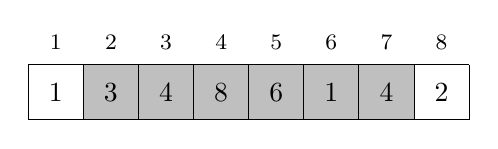
\begin{tikzpicture}[scale=0.7]
\fill[color=lightgray] (1,0) rectangle (7,1);
\draw (0,0) grid (8,1);

\node at (0.5,0.5) {$1$};
\node at (1.5,0.5) {$3$};
\node at (2.5,0.5) {$4$};
\node at (3.5,0.5) {$8$};
\node at (4.5,0.5) {$6$};
\node at (5.5,0.5) {$1$};
\node at (6.5,0.5) {$4$};
\node at (7.5,0.5) {$2$};

\footnotesize
\node at (0.5,1.4) {$1$};
\node at (1.5,1.4) {$2$};
\node at (2.5,1.4) {$3$};
\node at (3.5,1.4) {$4$};
\node at (4.5,1.4) {$5$};
\node at (5.5,1.4) {$6$};
\node at (6.5,1.4) {$7$};
\node at (7.5,1.4) {$8$};
\end{tikzpicture}
\end{center}
The length of the range $[2,7]$ is 6,
and $\lfloor \log_2(6) \rfloor = 2$.
Thus, the minimum can be calculated
from two ranges of length 4.
The ranges are $[2,5]$ and $[4,7]$:
\begin{center}
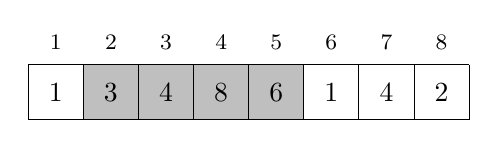
\begin{tikzpicture}[scale=0.7]
\fill[color=lightgray] (1,0) rectangle (5,1);
\draw (0,0) grid (8,1);

\node at (0.5,0.5) {$1$};
\node at (1.5,0.5) {$3$};
\node at (2.5,0.5) {$4$};
\node at (3.5,0.5) {$8$};
\node at (4.5,0.5) {$6$};
\node at (5.5,0.5) {$1$};
\node at (6.5,0.5) {$4$};
\node at (7.5,0.5) {$2$};

\footnotesize
\node at (0.5,1.4) {$1$};
\node at (1.5,1.4) {$2$};
\node at (2.5,1.4) {$3$};
\node at (3.5,1.4) {$4$};
\node at (4.5,1.4) {$5$};
\node at (5.5,1.4) {$6$};
\node at (6.5,1.4) {$7$};
\node at (7.5,1.4) {$8$};
\end{tikzpicture}
\end{center}
\begin{center}
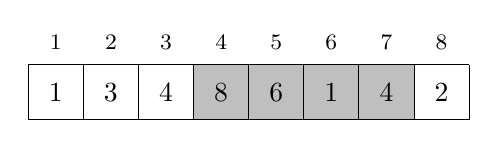
\begin{tikzpicture}[scale=0.7]
\fill[color=lightgray] (3,0) rectangle (7,1);
\draw (0,0) grid (8,1);

\node at (0.5,0.5) {$1$};
\node at (1.5,0.5) {$3$};
\node at (2.5,0.5) {$4$};
\node at (3.5,0.5) {$8$};
\node at (4.5,0.5) {$6$};
\node at (5.5,0.5) {$1$};
\node at (6.5,0.5) {$4$};
\node at (7.5,0.5) {$2$};


\footnotesize
\node at (0.5,1.4) {$1$};
\node at (1.5,1.4) {$2$};
\node at (2.5,1.4) {$3$};
\node at (3.5,1.4) {$4$};
\node at (4.5,1.4) {$5$};
\node at (5.5,1.4) {$6$};
\node at (6.5,1.4) {$7$};
\node at (7.5,1.4) {$8$};
\end{tikzpicture}
\end{center}
The minimum of the range $[2,5]$ is 3,
and the minimum of the range $[4,7]$ is 1.
Thus, the minimum of the range $[2,7]$ is 1.

\section{Binary indexed tree}

\index{binary indexed tree}
\index{Fenwick tree}

A \key{binary indexed tree} or a \key{Fenwick tree}
is a data structure that resembles a sum array.
The supported operations are answering
a sum query for range $[a,b]$,
and updating the element at index $k$.
The time complexity for both of the operations is $O(\log n)$.

Unlike a sum array, a binary indexed tree
can be efficiently updated between the sum queries.
This would not be possible using a sum array
because we should build the whole sum array again
in $O(n)$ time after each update.

\subsubsection{Structure}

A binary indexed tree can be represented as an array
where index $k$ contains the sum of a range in the
original array that ends to index $k$.
The length of the range is the largest power of two
that divides $k$.
For example, if $k=6$, the length of the range is $2$
because $2$ divides $6$ but $4$ doesn't divide $6$.

\begin{samepage}
For example, for the array
\begin{center}
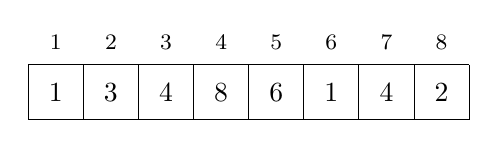
\begin{tikzpicture}[scale=0.7]
\draw (0,0) grid (8,1);

\node at (0.5,0.5) {$1$};
\node at (1.5,0.5) {$3$};
\node at (2.5,0.5) {$4$};
\node at (3.5,0.5) {$8$};
\node at (4.5,0.5) {$6$};
\node at (5.5,0.5) {$1$};
\node at (6.5,0.5) {$4$};
\node at (7.5,0.5) {$2$};

\footnotesize
\node at (0.5,1.4) {$1$};
\node at (1.5,1.4) {$2$};
\node at (2.5,1.4) {$3$};
\node at (3.5,1.4) {$4$};
\node at (4.5,1.4) {$5$};
\node at (5.5,1.4) {$6$};
\node at (6.5,1.4) {$7$};
\node at (7.5,1.4) {$8$};
\end{tikzpicture}
\end{center}
\end{samepage}
the corresponding binary indexed tree is as follows:
\begin{center}
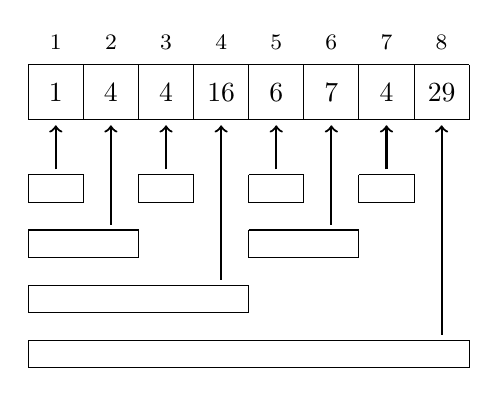
\begin{tikzpicture}[scale=0.7]
%\fill[color=lightgray] (3,0) rectangle (7,1);
\draw (0,0) grid (8,1);

\node at (0.5,0.5) {$1$};
\node at (1.5,0.5) {$4$};
\node at (2.5,0.5) {$4$};
\node at (3.5,0.5) {$16$};
\node at (4.5,0.5) {$6$};
\node at (5.5,0.5) {$7$};
\node at (6.5,0.5) {$4$};
\node at (7.5,0.5) {$29$};

\footnotesize
\node at (0.5,1.4) {$1$};
\node at (1.5,1.4) {$2$};
\node at (2.5,1.4) {$3$};
\node at (3.5,1.4) {$4$};
\node at (4.5,1.4) {$5$};
\node at (5.5,1.4) {$6$};
\node at (6.5,1.4) {$7$};
\node at (7.5,1.4) {$8$};

\draw[->,thick] (0.5,-0.9) -- (0.5,-0.1);
\draw[->,thick] (2.5,-0.9) -- (2.5,-0.1);
\draw[->,thick] (4.5,-0.9) -- (4.5,-0.1);
\draw[->,thick] (6.5,-0.9) -- (6.5,-0.1);
\draw[->,thick] (1.5,-1.9) -- (1.5,-0.1);
\draw[->,thick] (5.5,-1.9) -- (5.5,-0.1);
\draw[->,thick] (3.5,-2.9) -- (3.5,-0.1);
\draw[->,thick] (7.5,-3.9) -- (7.5,-0.1);

\draw (0,-1) -- (1,-1) -- (1,-1.5) -- (0,-1.5) -- (0,-1);
\draw (2,-1) -- (3,-1) -- (3,-1.5) -- (2,-1.5) -- (2,-1);
\draw (4,-1) -- (5,-1) -- (5,-1.5) -- (4,-1.5) -- (4,-1);
\draw (6,-1) -- (7,-1) -- (7,-1.5) -- (6,-1.5) -- (6,-1);
\draw (0,-2) -- (2,-2) -- (2,-2.5) -- (0,-2.5) -- (0,-2);
\draw (4,-2) -- (6,-2) -- (6,-2.5) -- (4,-2.5) -- (4,-2);
\draw (0,-3) -- (4,-3) -- (4,-3.5) -- (0,-3.5) -- (0,-3);
\draw (0,-4) -- (8,-4) -- (8,-4.5) -- (0,-4.5) -- (0,-4);
\end{tikzpicture}
\end{center}

For example, the binary indexed tree
contains the value 7 at index 6
because the sum of the elements in the range $[5,6]$
of the original array is $6+1=7$.

\subsubsection{Sum query}

The basic operation in a binary indexed tree is
calculating the sum of a range $[1,k]$ where $k$
is any index in the array.
The sum of any range can be constructed by combining
sums of subranges in the tree.

For example, the range $[1,7]$ will be divided
into three subranges:
\begin{center}
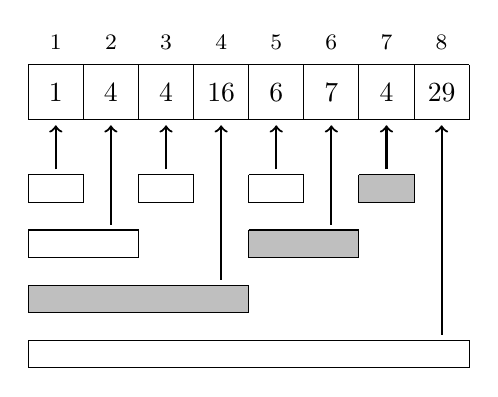
\begin{tikzpicture}[scale=0.7]
%\fill[color=lightgray] (3,0) rectangle (7,1);
\draw (0,0) grid (8,1);

\node at (0.5,0.5) {$1$};
\node at (1.5,0.5) {$4$};
\node at (2.5,0.5) {$4$};
\node at (3.5,0.5) {$16$};
\node at (4.5,0.5) {$6$};
\node at (5.5,0.5) {$7$};
\node at (6.5,0.5) {$4$};
\node at (7.5,0.5) {$29$};

\footnotesize
\node at (0.5,1.4) {$1$};
\node at (1.5,1.4) {$2$};
\node at (2.5,1.4) {$3$};
\node at (3.5,1.4) {$4$};
\node at (4.5,1.4) {$5$};
\node at (5.5,1.4) {$6$};
\node at (6.5,1.4) {$7$};
\node at (7.5,1.4) {$8$};

\draw[->,thick] (0.5,-0.9) -- (0.5,-0.1);
\draw[->,thick] (2.5,-0.9) -- (2.5,-0.1);
\draw[->,thick] (4.5,-0.9) -- (4.5,-0.1);
\draw[->,thick] (6.5,-0.9) -- (6.5,-0.1);
\draw[->,thick] (1.5,-1.9) -- (1.5,-0.1);
\draw[->,thick] (5.5,-1.9) -- (5.5,-0.1);
\draw[->,thick] (3.5,-2.9) -- (3.5,-0.1);
\draw[->,thick] (7.5,-3.9) -- (7.5,-0.1);

\draw (0,-1) -- (1,-1) -- (1,-1.5) -- (0,-1.5) -- (0,-1);
\draw (2,-1) -- (3,-1) -- (3,-1.5) -- (2,-1.5) -- (2,-1);
\draw (4,-1) -- (5,-1) -- (5,-1.5) -- (4,-1.5) -- (4,-1);
\draw[fill=lightgray] (6,-1) -- (7,-1) -- (7,-1.5) -- (6,-1.5) -- (6,-1);
\draw (0,-2) -- (2,-2) -- (2,-2.5) -- (0,-2.5) -- (0,-2);
\draw[fill=lightgray] (4,-2) -- (6,-2) -- (6,-2.5) -- (4,-2.5) -- (4,-2);
\draw[fill=lightgray] (0,-3) -- (4,-3) -- (4,-3.5) -- (0,-3.5) -- (0,-3);
\draw (0,-4) -- (8,-4) -- (8,-4.5) -- (0,-4.5) -- (0,-4);
\end{tikzpicture}
\end{center}

Thus, the sum of the range $[1,7]$ is $16+7+4=27$.
Because of the structure of the binary indexed tree,
the length of each subrange inside a range is distinct,
so the sum of a range
always consists of sums of $O(\log n)$ subranges.

Using the same technique that we previously used
with a sum array,
we can efficiently calculate the sum of any range
$[a,b]$ by substracting the sum of the range $[1,a-1]$
from the sum of the range $[1,b]$.
The time complexity remains $O(\log n)$
because it suffices to calculate two sums of $[1,k]$ ranges.

\subsubsection{Array update}

When an element in the original array changes,
several sums in the binary indexed tree change.
For example, if the value at index 3 changes,
the sums of the following ranges change:
\begin{center}
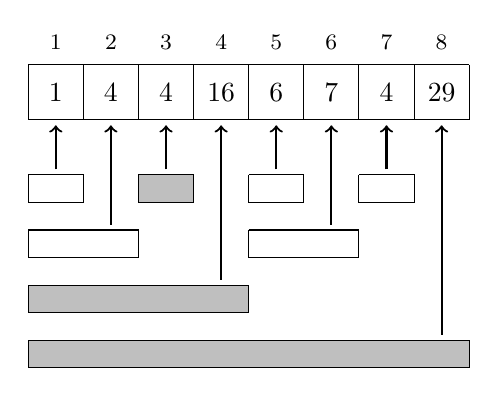
\begin{tikzpicture}[scale=0.7]
%\fill[color=lightgray] (3,0) rectangle (7,1);
\draw (0,0) grid (8,1);

\node at (0.5,0.5) {$1$};
\node at (1.5,0.5) {$4$};
\node at (2.5,0.5) {$4$};
\node at (3.5,0.5) {$16$};
\node at (4.5,0.5) {$6$};
\node at (5.5,0.5) {$7$};
\node at (6.5,0.5) {$4$};
\node at (7.5,0.5) {$29$};

\footnotesize
\node at (0.5,1.4) {$1$};
\node at (1.5,1.4) {$2$};
\node at (2.5,1.4) {$3$};
\node at (3.5,1.4) {$4$};
\node at (4.5,1.4) {$5$};
\node at (5.5,1.4) {$6$};
\node at (6.5,1.4) {$7$};
\node at (7.5,1.4) {$8$};

\draw[->,thick] (0.5,-0.9) -- (0.5,-0.1);
\draw[->,thick] (2.5,-0.9) -- (2.5,-0.1);
\draw[->,thick] (4.5,-0.9) -- (4.5,-0.1);
\draw[->,thick] (6.5,-0.9) -- (6.5,-0.1);
\draw[->,thick] (1.5,-1.9) -- (1.5,-0.1);
\draw[->,thick] (5.5,-1.9) -- (5.5,-0.1);
\draw[->,thick] (3.5,-2.9) -- (3.5,-0.1);
\draw[->,thick] (7.5,-3.9) -- (7.5,-0.1);

\draw (0,-1) -- (1,-1) -- (1,-1.5) -- (0,-1.5) -- (0,-1);
\draw[fill=lightgray] (2,-1) -- (3,-1) -- (3,-1.5) -- (2,-1.5) -- (2,-1);
\draw (4,-1) -- (5,-1) -- (5,-1.5) -- (4,-1.5) -- (4,-1);
\draw (6,-1) -- (7,-1) -- (7,-1.5) -- (6,-1.5) -- (6,-1);
\draw (0,-2) -- (2,-2) -- (2,-2.5) -- (0,-2.5) -- (0,-2);
\draw (4,-2) -- (6,-2) -- (6,-2.5) -- (4,-2.5) -- (4,-2);
\draw[fill=lightgray] (0,-3) -- (4,-3) -- (4,-3.5) -- (0,-3.5) -- (0,-3);
\draw[fill=lightgray] (0,-4) -- (8,-4) -- (8,-4.5) -- (0,-4.5) -- (0,-4);
\end{tikzpicture}
\end{center}

Also in this case, the length of each range is distinct,
so $O(\log n)$ ranges will be updated in the binary indexed tree.

\subsubsection{Implementation}

The operations of a binary indexed tree can be implemented
in an elegant and efficient way using bit manipulation.
The bit operation needed is $k \& -k$ that
returns the last bit one from number $k$.
For example, $6 \& -6=2$ because the number $6$
corresponds to 110 and the number $2$ corresponds to 10.

It turns out that when calculating a range sum,
the index $k$ in the binary indexed tree should be
decreased by $k \& -k$ at every step.
Correspondingly, when updating the array,
the index $k$ should be increased by $k \& -k$ at every step.

The following functions assume that the binary indexed tree
is stored to array \texttt{b} and it consists of indices $1 \ldots n$.

The function \texttt{sum} calculates the sum of the range $[1,k]$:
\begin{lstlisting}
int sum(int k) {
    int s = 0;
    while (k >= 1) {
        s += b[k];
        k -= k&-k;
    }
    return s;
}
\end{lstlisting}

The function \texttt{add} increases the value of element $k$ by $x$:
\begin{lstlisting}
void add(int k, int x) {
    while (k <= n) {
        b[k] += x;
        k += k&-k;
    }
}
\end{lstlisting}

The time complexity of both above functions is
$O(\log n)$ because the functions change $O(\log n)$
values in the binary indexed tree and each move
to the next index
takes $O(1)$ time using the bit operation.

\section{Segment tree}

\index{segment tree}

A \key{segment tree} is a data structure
whose supported operations are
handling a range query for range $[a,b]$
and updating the element at index $k$.
Using a segment tree, we can implement sum
queries, minimum queries and many other
queries so that both operations work in $O(\log n)$ time.

Compared to a binary indexed tree,
the advantage of a segment tree is that it is
a more general data structure.
While binary indexed trees only support
sum queries, segment trees also support other queries.
On the other hand, a segment tree requires more
memory and is a bit more difficult to implement.

\subsubsection{Structure}

A segment tree contains $2n-1$ nodes
so that the bottom $n$ nodes correspond
to the original array and the other nodes
contain information needed for range queries.
The values in a segment tree depend on
the supported query type.
We will first assume that the supported
query is the sum query.

For example, the array
\begin{center}
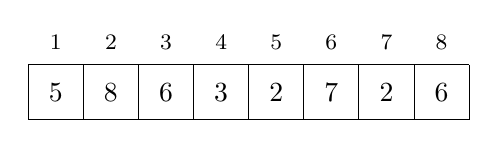
\begin{tikzpicture}[scale=0.7]
\draw (0,0) grid (8,1);

\node at (0.5,0.5) {$5$};
\node at (1.5,0.5) {$8$};
\node at (2.5,0.5) {$6$};
\node at (3.5,0.5) {$3$};
\node at (4.5,0.5) {$2$};
\node at (5.5,0.5) {$7$};
\node at (6.5,0.5) {$2$};
\node at (7.5,0.5) {$6$};

\footnotesize
\node at (0.5,1.4) {$1$};
\node at (1.5,1.4) {$2$};
\node at (2.5,1.4) {$3$};
\node at (3.5,1.4) {$4$};
\node at (4.5,1.4) {$5$};
\node at (5.5,1.4) {$6$};
\node at (6.5,1.4) {$7$};
\node at (7.5,1.4) {$8$};
\end{tikzpicture}
\end{center}
corresponds to the following segment tree:
\begin{center}
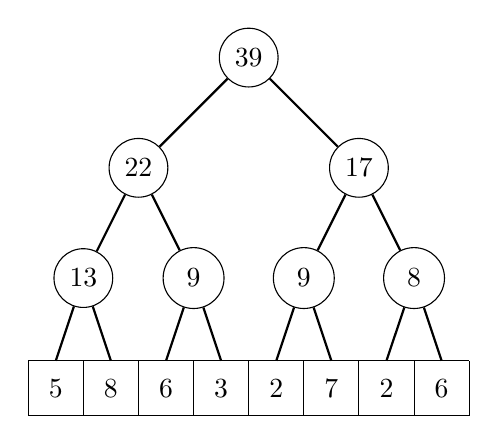
\begin{tikzpicture}[scale=0.7]
\draw (0,0) grid (8,1);

\node[anchor=center] at (0.5, 0.5) {5};
\node[anchor=center] at (1.5, 0.5) {8};
\node[anchor=center] at (2.5, 0.5) {6};
\node[anchor=center] at (3.5, 0.5) {3};
\node[anchor=center] at (4.5, 0.5) {2};
\node[anchor=center] at (5.5, 0.5) {7};
\node[anchor=center] at (6.5, 0.5) {2};
\node[anchor=center] at (7.5, 0.5) {6};

\node[draw, circle] (a) at (1,2.5) {13};
\path[draw,thick,-] (a) -- (0.5,1);
\path[draw,thick,-] (a) -- (1.5,1);
\node[draw, circle,minimum size=22pt] (b) at (3,2.5) {9};
\path[draw,thick,-] (b) -- (2.5,1);
\path[draw,thick,-] (b) -- (3.5,1);
\node[draw, circle,minimum size=22pt] (c) at (5,2.5) {9};
\path[draw,thick,-] (c) -- (4.5,1);
\path[draw,thick,-] (c) -- (5.5,1);
\node[draw, circle,minimum size=22pt] (d) at (7,2.5) {8};
\path[draw,thick,-] (d) -- (6.5,1);
\path[draw,thick,-] (d) -- (7.5,1);

\node[draw, circle] (i) at (2,4.5) {22};
\path[draw,thick,-] (i) -- (a);
\path[draw,thick,-] (i) -- (b);
\node[draw, circle] (j) at (6,4.5) {17};
\path[draw,thick,-] (j) -- (c);
\path[draw,thick,-] (j) -- (d);

\node[draw, circle] (m) at (4,6.5) {39};
\path[draw,thick,-] (m) -- (i);
\path[draw,thick,-] (m) -- (j);
\end{tikzpicture}
\end{center}

Each internal node in the segment tree contains
information about a range of size $2^k$
in the original array.
In the above tree, the value of each internal
node is the sum of the corresponding array elements,
and it can be calculated as the sum of
the values of its left and right child node.

It is convenient to build a segment tree
when the size of the array is a power of two
and the tree is a complete binary tree.
In the sequel, we will assume that the tree
is built like this.
If the size of the array is not a power of two,
we can always extend it using zero elements.

\subsubsection{Range query}

In a segment tree, the answer for a range query
is calculated from nodes that belong to the range
and are as high as possible in the tree.
Each node gives the answer for a subrange,
and the answer for the entire range can be
calculated by combining these values.

For example, consider the following range:
\begin{center}
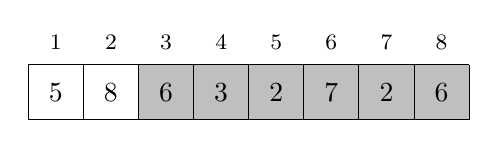
\begin{tikzpicture}[scale=0.7]
\fill[color=gray!50] (2,0) rectangle (8,1);
\draw (0,0) grid (8,1);

\node[anchor=center] at (0.5, 0.5) {5};
\node[anchor=center] at (1.5, 0.5) {8};
\node[anchor=center] at (2.5, 0.5) {6};
\node[anchor=center] at (3.5, 0.5) {3};
\node[anchor=center] at (4.5, 0.5) {2};
\node[anchor=center] at (5.5, 0.5) {7};
\node[anchor=center] at (6.5, 0.5) {2};
\node[anchor=center] at (7.5, 0.5) {6};

\footnotesize
\node at (0.5,1.4) {$1$};
\node at (1.5,1.4) {$2$};
\node at (2.5,1.4) {$3$};
\node at (3.5,1.4) {$4$};
\node at (4.5,1.4) {$5$};
\node at (5.5,1.4) {$6$};
\node at (6.5,1.4) {$7$};
\node at (7.5,1.4) {$8$};
\end{tikzpicture}
\end{center}
The sum of elements in the range $[3,8]$ is
$6+3+2+7+2+6=26$.
The sum can be calculated from the segment tree
using the following subranges:
\begin{center}
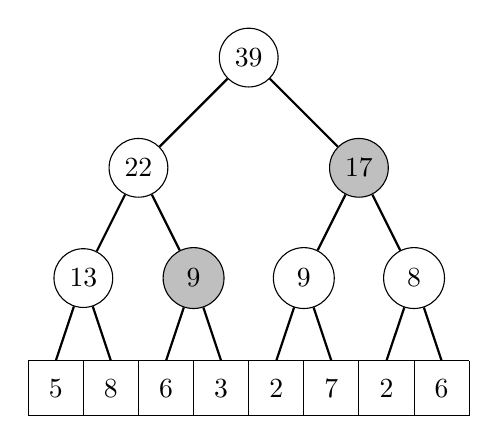
\begin{tikzpicture}[scale=0.7]
\draw (0,0) grid (8,1);

\node[anchor=center] at (0.5, 0.5) {5};
\node[anchor=center] at (1.5, 0.5) {8};
\node[anchor=center] at (2.5, 0.5) {6};
\node[anchor=center] at (3.5, 0.5) {3};
\node[anchor=center] at (4.5, 0.5) {2};
\node[anchor=center] at (5.5, 0.5) {7};
\node[anchor=center] at (6.5, 0.5) {2};
\node[anchor=center] at (7.5, 0.5) {6};

\node[draw, circle] (a) at (1,2.5) {13};
\path[draw,thick,-] (a) -- (0.5,1);
\path[draw,thick,-] (a) -- (1.5,1);
\node[draw, circle,fill=gray!50,minimum size=22pt] (b) at (3,2.5) {9};
\path[draw,thick,-] (b) -- (2.5,1);
\path[draw,thick,-] (b) -- (3.5,1);
\node[draw, circle,minimum size=22pt] (c) at (5,2.5) {9};
\path[draw,thick,-] (c) -- (4.5,1);
\path[draw,thick,-] (c) -- (5.5,1);
\node[draw, circle,minimum size=22pt] (d) at (7,2.5) {8};
\path[draw,thick,-] (d) -- (6.5,1);
\path[draw,thick,-] (d) -- (7.5,1);

\node[draw, circle] (i) at (2,4.5) {22};
\path[draw,thick,-] (i) -- (a);
\path[draw,thick,-] (i) -- (b);
\node[draw, circle,fill=gray!50] (j) at (6,4.5) {17};
\path[draw,thick,-] (j) -- (c);
\path[draw,thick,-] (j) -- (d);

\node[draw, circle] (m) at (4,6.5) {39};
\path[draw,thick,-] (m) -- (i);
\path[draw,thick,-] (m) -- (j);
\end{tikzpicture}
\end{center}
Thus, the sum of the range is $9+17=26$.

When the answer for a range query is
calculated using as high nodes as possible,
at most two nodes on each level
of the segment tree are needed.
Because of this, the total number of nodes
examined is only $O(\log n)$.

\subsubsection{Array update}

When an element in the array changes,
we should update all nodes in the segment tree
whose value depends on the changed element.
This can be done by travelling from the bottom
to the top in the tree and updating the nodes along the path.

\begin{samepage}
The following picture shows which nodes in the segment tree
change if the element 7 in the array changes.

\begin{center}
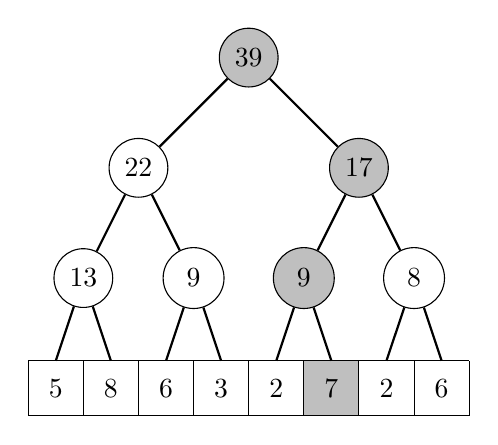
\begin{tikzpicture}[scale=0.7]
\fill[color=gray!50] (5,0) rectangle (6,1);
\draw (0,0) grid (8,1);

\node[anchor=center] at (0.5, 0.5) {5};
\node[anchor=center] at (1.5, 0.5) {8};
\node[anchor=center] at (2.5, 0.5) {6};
\node[anchor=center] at (3.5, 0.5) {3};
\node[anchor=center] at (4.5, 0.5) {2};
\node[anchor=center] at (5.5, 0.5) {7};
\node[anchor=center] at (6.5, 0.5) {2};
\node[anchor=center] at (7.5, 0.5) {6};

\node[draw, circle] (a) at (1,2.5) {13};
\path[draw,thick,-] (a) -- (0.5,1);
\path[draw,thick,-] (a) -- (1.5,1);
\node[draw, circle,minimum size=22pt] (b) at (3,2.5) {9};
\path[draw,thick,-] (b) -- (2.5,1);
\path[draw,thick,-] (b) -- (3.5,1);
\node[draw, circle,minimum size=22pt,fill=gray!50] (c) at (5,2.5) {9};
\path[draw,thick,-] (c) -- (4.5,1);
\path[draw,thick,-] (c) -- (5.5,1);
\node[draw, circle,minimum size=22pt] (d) at (7,2.5) {8};
\path[draw,thick,-] (d) -- (6.5,1);
\path[draw,thick,-] (d) -- (7.5,1);

\node[draw, circle] (i) at (2,4.5) {22};
\path[draw,thick,-] (i) -- (a);
\path[draw,thick,-] (i) -- (b);
\node[draw, circle,fill=gray!50] (j) at (6,4.5) {17};
\path[draw,thick,-] (j) -- (c);
\path[draw,thick,-] (j) -- (d);

\node[draw, circle,fill=gray!50] (m) at (4,6.5) {39};
\path[draw,thick,-] (m) -- (i);
\path[draw,thick,-] (m) -- (j);
\end{tikzpicture}
\end{center}
\end{samepage}

The path from the bottom of the segment tree to the top
always consists of $O(\log n)$ nodes,
so updating the array affects $O(\log n)$ nodes in the tree.

\subsubsection{Storing the tree}

A segment tree can be stored as an array
of $2N$ elements where $N$ is a power of two.
From now on, we will assume that the indices
of the original array are between $0$ and $N-1$.

The element at index 1 in the segment tree array
contains the top node of the tree,
the elements at indices 2 and 3 correspond to
the second level of the tree, and so on.
Finally, the elements beginning from index $N$
contain the bottom level of the tree, i.e.,
the actual content of the original array.

For example, the segment tree
\begin{center}
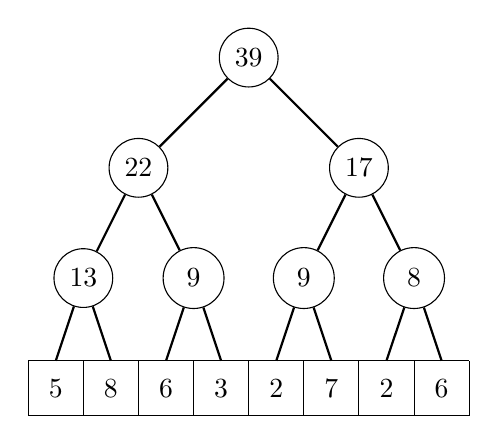
\begin{tikzpicture}[scale=0.7]
\draw (0,0) grid (8,1);

\node[anchor=center] at (0.5, 0.5) {5};
\node[anchor=center] at (1.5, 0.5) {8};
\node[anchor=center] at (2.5, 0.5) {6};
\node[anchor=center] at (3.5, 0.5) {3};
\node[anchor=center] at (4.5, 0.5) {2};
\node[anchor=center] at (5.5, 0.5) {7};
\node[anchor=center] at (6.5, 0.5) {2};
\node[anchor=center] at (7.5, 0.5) {6};

\node[draw, circle] (a) at (1,2.5) {13};
\path[draw,thick,-] (a) -- (0.5,1);
\path[draw,thick,-] (a) -- (1.5,1);
\node[draw, circle,minimum size=22pt] (b) at (3,2.5) {9};
\path[draw,thick,-] (b) -- (2.5,1);
\path[draw,thick,-] (b) -- (3.5,1);
\node[draw, circle,minimum size=22pt] (c) at (5,2.5) {9};
\path[draw,thick,-] (c) -- (4.5,1);
\path[draw,thick,-] (c) -- (5.5,1);
\node[draw, circle,minimum size=22pt] (d) at (7,2.5) {8};
\path[draw,thick,-] (d) -- (6.5,1);
\path[draw,thick,-] (d) -- (7.5,1);

\node[draw, circle] (i) at (2,4.5) {22};
\path[draw,thick,-] (i) -- (a);
\path[draw,thick,-] (i) -- (b);
\node[draw, circle] (j) at (6,4.5) {17};
\path[draw,thick,-] (j) -- (c);
\path[draw,thick,-] (j) -- (d);

\node[draw, circle] (m) at (4,6.5) {39};
\path[draw,thick,-] (m) -- (i);
\path[draw,thick,-] (m) -- (j);
\end{tikzpicture}
\end{center}
can be stored as follows ($N=8$):
\begin{center}
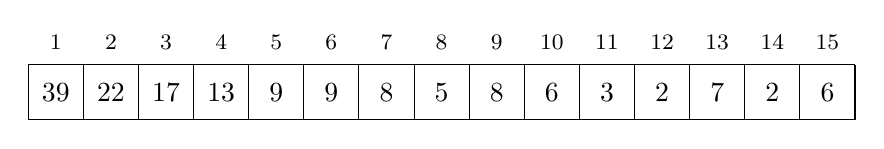
\begin{tikzpicture}[scale=0.7]
%\fill[color=lightgray] (3,0) rectangle (7,1);
\draw (0,0) grid (15,1);

\node at (0.5,0.5) {$39$};
\node at (1.5,0.5) {$22$};
\node at (2.5,0.5) {$17$};
\node at (3.5,0.5) {$13$};
\node at (4.5,0.5) {$9$};
\node at (5.5,0.5) {$9$};
\node at (6.5,0.5) {$8$};
\node at (7.5,0.5) {$5$};
\node at (8.5,0.5) {$8$};
\node at (9.5,0.5) {$6$};
\node at (10.5,0.5) {$3$};
\node at (11.5,0.5) {$2$};
\node at (12.5,0.5) {$7$};
\node at (13.5,0.5) {$2$};
\node at (14.5,0.5) {$6$};

\footnotesize
\node at (0.5,1.4) {$1$};
\node at (1.5,1.4) {$2$};
\node at (2.5,1.4) {$3$};
\node at (3.5,1.4) {$4$};
\node at (4.5,1.4) {$5$};
\node at (5.5,1.4) {$6$};
\node at (6.5,1.4) {$7$};
\node at (7.5,1.4) {$8$};
\node at (8.5,1.4) {$9$};
\node at (9.5,1.4) {$10$};
\node at (10.5,1.4) {$11$};
\node at (11.5,1.4) {$12$};
\node at (12.5,1.4) {$13$};
\node at (13.5,1.4) {$14$};
\node at (14.5,1.4) {$15$};
\end{tikzpicture}
\end{center}
Using this representation,
for a node at index $k$,
\begin{itemize}
\item the parent node is at index $\lfloor k/2 \rfloor$,
\item the left child node is at index $2k$, and
\item the right child node is at index $2k+1$.
\end{itemize}
Note that this implies that the index of a node
is even if it is a left child and odd if it is a right child.

\subsubsection{Functions}

We assume that the segment tree is stored
in the array \texttt{p}.
The following function calculates the sum of range $[a,b]$:

\begin{lstlisting}
int sum(int a, int b) {
    a += N; b += N;
    int s = 0;
    while (a <= b) {
        if (a%2 == 1) s += p[a++];
        if (b%2 == 0) s += p[b--];
        a /= 2; b /= 2;
    }
    return s;
}
\end{lstlisting}

The function begins from the bottom of the tree
and moves step by step upwards in the tree.
The function calculates the range sum to
the variable $s$ by combining the sums in the tree nodes.
The value of a node is added to the sum if
the parent node doesn't belong to the range.

The function \texttt{add} increases the value
of element $k$ by $x$:

\begin{lstlisting}
void add(int k, int x) {
    k += N;
    p[k] += x;
    for (k /= 2; k >= 1; k /= 2) {
        p[k] = p[2*k]+p[2*k+1];
    }
}
\end{lstlisting}
First the function updates the bottom level
of the tree that corresponds to the original array.
After this, the function updates the values of all
internal nodes in the tree, until it reaches
the root node of the tree.

Both operations in the segment tree work
in $O(\log n)$ time because a segment tree
of $n$ elements consists of $O(\log n)$ levels,
and the operations move one level forward at each step.

\subsubsection{Other queries}

Besides the sum query,
the segment tree can support any range query
where the answer for range $[a,b]$
can be efficiently calculated
from ranges $[a,c]$ and $[c+1,b]$ where
$c$ is some element between $a$ and $b$.
Such queries are, for example,
minimum and maximum, greatest common divisor,
and bit operations.

\begin{samepage}
For example, the following segment tree
supports minimum queries:

\begin{center}
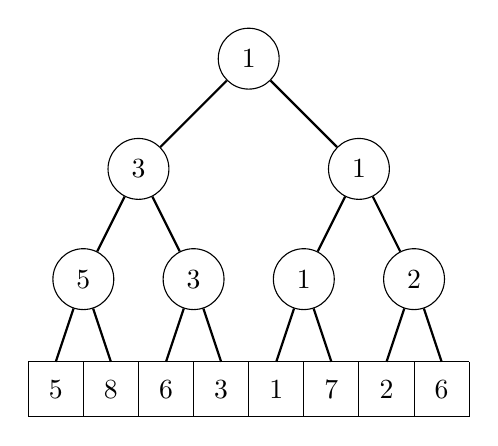
\begin{tikzpicture}[scale=0.7]
\draw (0,0) grid (8,1);

\node[anchor=center] at (0.5, 0.5) {5};
\node[anchor=center] at (1.5, 0.5) {8};
\node[anchor=center] at (2.5, 0.5) {6};
\node[anchor=center] at (3.5, 0.5) {3};
\node[anchor=center] at (4.5, 0.5) {1};
\node[anchor=center] at (5.5, 0.5) {7};
\node[anchor=center] at (6.5, 0.5) {2};
\node[anchor=center] at (7.5, 0.5) {6};

\node[draw, circle,minimum size=22pt] (a) at (1,2.5) {5};
\path[draw,thick,-] (a) -- (0.5,1);
\path[draw,thick,-] (a) -- (1.5,1);
\node[draw, circle,minimum size=22pt] (b) at (3,2.5) {3};
\path[draw,thick,-] (b) -- (2.5,1);
\path[draw,thick,-] (b) -- (3.5,1);
\node[draw, circle,minimum size=22pt] (c) at (5,2.5) {1};
\path[draw,thick,-] (c) -- (4.5,1);
\path[draw,thick,-] (c) -- (5.5,1);
\node[draw, circle,minimum size=22pt] (d) at (7,2.5) {2};
\path[draw,thick,-] (d) -- (6.5,1);
\path[draw,thick,-] (d) -- (7.5,1);

\node[draw, circle,minimum size=22pt] (i) at (2,4.5) {3};
\path[draw,thick,-] (i) -- (a);
\path[draw,thick,-] (i) -- (b);
\node[draw, circle,minimum size=22pt] (j) at (6,4.5) {1};
\path[draw,thick,-] (j) -- (c);
\path[draw,thick,-] (j) -- (d);

\node[draw, circle,minimum size=22pt] (m) at (4,6.5) {1};
\path[draw,thick,-] (m) -- (i);
\path[draw,thick,-] (m) -- (j);
\end{tikzpicture}
\end{center}
\end{samepage}

In this segment tree, every node in the tree
contains the smallest element in the corresponding
range of the original array.
The top node of the tree contains the smallest
element in the array.
The tree can be implemented like previously,
but instead of sums, minima are calculated.

\subsubsection{Binary search in tree}

The structure of the segment tree makes it possible
to use binary search.
For example, if the tree supports the minimum query,
we can find the index of the smallest
element in $O(\log n)$ time.

For example, in the following tree the
smallest element is 1 that can be found
by following a path downwards from the top node:

\begin{center}
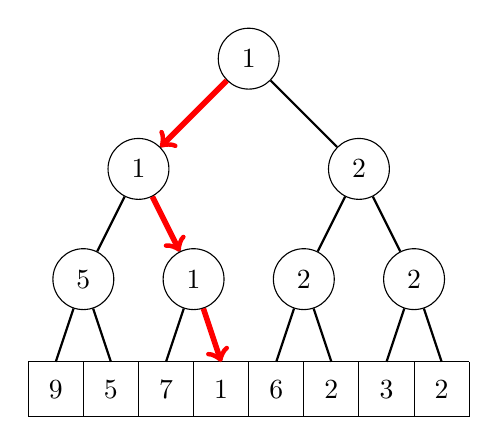
\begin{tikzpicture}[scale=0.7]
\draw (8,0) grid (16,1);

\node[anchor=center] at (8.5, 0.5) {9};
\node[anchor=center] at (9.5, 0.5) {5};
\node[anchor=center] at (10.5, 0.5) {7};
\node[anchor=center] at (11.5, 0.5) {1};
\node[anchor=center] at (12.5, 0.5) {6};
\node[anchor=center] at (13.5, 0.5) {2};
\node[anchor=center] at (14.5, 0.5) {3};
\node[anchor=center] at (15.5, 0.5) {2};

%\node[anchor=center] at (1,2.5) {13};

\node[draw, circle,minimum size=22pt] (e) at (9,2.5) {5};
\path[draw,thick,-] (e) -- (8.5,1);
\path[draw,thick,-] (e) -- (9.5,1);
\node[draw, circle,minimum size=22pt] (f) at (11,2.5) {1};
\path[draw,thick,-] (f) -- (10.5,1);
\path[draw,thick,-] (f) -- (11.5,1);
\node[draw, circle,minimum size=22pt] (g) at (13,2.5) {2};
\path[draw,thick,-] (g) -- (12.5,1);
\path[draw,thick,-] (g) -- (13.5,1);
\node[draw, circle,minimum size=22pt] (h) at (15,2.5) {2};
\path[draw,thick,-] (h) -- (14.5,1);
\path[draw,thick,-] (h) -- (15.5,1);

\node[draw, circle,minimum size=22pt] (k) at (10,4.5) {1};
\path[draw,thick,-] (k) -- (e);
\path[draw,thick,-] (k) -- (f);
\node[draw, circle,minimum size=22pt] (l) at (14,4.5) {2};
\path[draw,thick,-] (l) -- (g);
\path[draw,thick,-] (l) -- (h);

\node[draw, circle,minimum size=22pt] (n) at (12,6.5) {1};
\path[draw,thick,-] (n) -- (k);
\path[draw,thick,-] (n) -- (l);


\path[draw=red,thick,->,line width=2pt] (n) -- (k);
\path[draw=red,thick,->,line width=2pt] (k) -- (f);
\path[draw=red,thick,->,line width=2pt] (f) -- (11.5,1);
\end{tikzpicture}
\end{center}

\section{Additional techniques}

\subsubsection{Index compression}

A limitation in data structures that have
been built upon an array is that
the elements are indexed using integers
$1,2,3,$ etc.
Difficulties arise when the indices
needed are large.
For example, using the index $10^9$ would
require that the array would contain $10^9$
elements which is not realistic.

\index{index compression}

However, we can often bypass this limitation
by using \key{index compression}
where the indices are redistributed so that
they are integers $1,2,3,$ etc.
This can be done if we know all the indices
needed during the algorithm beforehand.

The idea is to replace each original index $x$
with index $p(x)$ where $p$ is a function that
redistributes the indices.
We require that the order of the indices
doesn't change, so if $a<b$, then $p(a)<p(b)$.
Thanks to this, we can conviently perform queries
despite the fact that the indices are compressed.

For example, if the original indices are
$555$, $10^9$ and $8$, the new indices are:

\[
\begin{array}{lcl}
p(8) & = & 1 \\
p(555) & = & 2 \\
p(10^9) & = & 3 \\
\end{array}
\]

\subsubsection{Range update}

So far, we have implemented data structures
that support range queries and modifications
of single values.
Let us now consider a reverse situation
where we should update ranges and
retrieve single values.
We focus on an operation that increases all
elements in range $[a,b]$ by $x$.

Surprisingly, we can use the data structures
presented in this chapter also in this situation.
This requires that we change the array so that
each element indicates the \emph{change}
with respect to the previous element.
For example, the array

\begin{center}
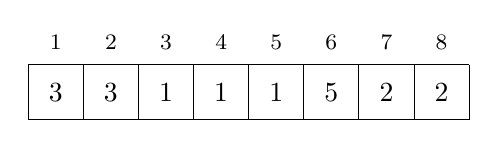
\begin{tikzpicture}[scale=0.7]
\draw (0,0) grid (8,1);

\node at (0.5,0.5) {$3$};
\node at (1.5,0.5) {$3$};
\node at (2.5,0.5) {$1$};
\node at (3.5,0.5) {$1$};
\node at (4.5,0.5) {$1$};
\node at (5.5,0.5) {$5$};
\node at (6.5,0.5) {$2$};
\node at (7.5,0.5) {$2$};


\footnotesize
\node at (0.5,1.4) {$1$};
\node at (1.5,1.4) {$2$};
\node at (2.5,1.4) {$3$};
\node at (3.5,1.4) {$4$};
\node at (4.5,1.4) {$5$};
\node at (5.5,1.4) {$6$};
\node at (6.5,1.4) {$7$};
\node at (7.5,1.4) {$8$};
\end{tikzpicture}
\end{center}
becomes as follows:
\begin{center}
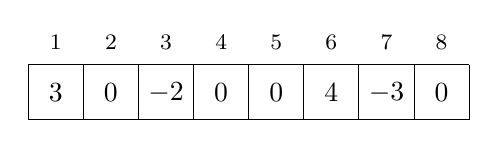
\begin{tikzpicture}[scale=0.7]
\draw (0,0) grid (8,1);

\node at (0.5,0.5) {$3$};
\node at (1.5,0.5) {$0$};
\node at (2.5,0.5) {$-2$};
\node at (3.5,0.5) {$0$};
\node at (4.5,0.5) {$0$};
\node at (5.5,0.5) {$4$};
\node at (6.5,0.5) {$-3$};
\node at (7.5,0.5) {$0$};


\footnotesize
\node at (0.5,1.4) {$1$};
\node at (1.5,1.4) {$2$};
\node at (2.5,1.4) {$3$};
\node at (3.5,1.4) {$4$};
\node at (4.5,1.4) {$5$};
\node at (5.5,1.4) {$6$};
\node at (6.5,1.4) {$7$};
\node at (7.5,1.4) {$8$};
\end{tikzpicture}
\end{center}

The original array is the sum array of the new array.
Thus, any value in the original array corresponds
to a sum of elements in the new array.
For example, the value 6 at index 5 in the original array
corresponds to the sum $3-2+4=5$.

The benefit in using the new array is
that we can update a range by changing just
two elements in the new array.
For example, if we want to 
increase the range $2 \ldots 5$ by 5,
it suffices to increase the element at index 2 by 5
and decrease the element at index 6 by 5.
The result is as follows:

\begin{center}
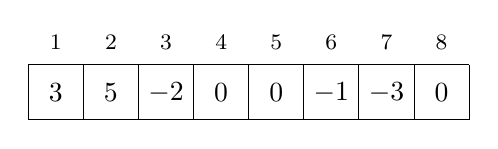
\begin{tikzpicture}[scale=0.7]
\draw (0,0) grid (8,1);

\node at (0.5,0.5) {$3$};
\node at (1.5,0.5) {$5$};
\node at (2.5,0.5) {$-2$};
\node at (3.5,0.5) {$0$};
\node at (4.5,0.5) {$0$};
\node at (5.5,0.5) {$-1$};
\node at (6.5,0.5) {$-3$};
\node at (7.5,0.5) {$0$};

\footnotesize
\node at (0.5,1.4) {$1$};
\node at (1.5,1.4) {$2$};
\node at (2.5,1.4) {$3$};
\node at (3.5,1.4) {$4$};
\node at (4.5,1.4) {$5$};
\node at (5.5,1.4) {$6$};
\node at (6.5,1.4) {$7$};
\node at (7.5,1.4) {$8$};
\end{tikzpicture}
\end{center}

More generally, to increase the range
$a \ldots b$ by $x$,
we increase the element at index $a$ by $x$
and decrease the element at index $b+1$ by $x$.
The required operations are calculating
the sum in a range and updating a value,
so we can use a binary indexed tree or a segment tree.

A more difficult problem is to support both
range queries and range updates.
In Chapter 28 we will see that this is possible
as well.



